\documentclass[tikz,border=6pt]{standalone}

% общий стиль (подключается через TEXINPUTS)
% tikz-style.tex (общий стиль для всех TikZ-картинок)
\RequirePackage[T1,T2A]{fontenc}
\RequirePackage[utf8]{inputenc}

% Palatino-подобный шрифт (как в MathJax часто воспринимается «более вытянутым»)
\RequirePackage{txfonts}
% txfonts даёт предупреждение по кириллице (T2A/txr не определён).
% Оставляем txfonts для математики, а текстовый шрифт возвращаем на Computer Modern,
% чтобы не искать T2A/txr и убрать предупреждения.
\renewcommand{\rmdefault}{cmr}
\renewcommand{\sfdefault}{cmss}
\renewcommand{\ttdefault}{cmtt}

\RequirePackage{tikz}
\RequirePackage{xcolor}
\usetikzlibrary{calc}

% цвета
\definecolor{lightgreen}{RGB}{214,234,214}
\definecolor{darkgreen}{HTML}{0B7A0B}
\definecolor{darkred}{HTML}{DF0000}

\definecolor{midgreen}{HTML}{2E9B2E}
\definecolor{palegreen}{RGB}{235,246,235}
\definecolor{olivegreen}{HTML}{3E6B2F}

\definecolor{lightred}{RGB}{255,220,220}
\definecolor{midred}{HTML}{E04545}
\definecolor{darkred2}{HTML}{A80000}

\definecolor{lightblue}{RGB}{220,232,255}
\definecolor{midblue}{HTML}{2E5BD6}
\definecolor{darkblue}{HTML}{0B2E8A}

\definecolor{lightgray}{RGB}{240,240,240}
\definecolor{midgray}{RGB}{170,170,170}
\definecolor{darkgray}{RGB}{80,80,80}

\definecolor{vtxfill}{RGB}{86,193,255}
\definecolor{vennfill}{RGB}{220,232,255}


% единый набор стилей TikZ
\tikzset{
    lab/.style={
        font=\fontsize{24}{32}\selectfont
    }
}


\begin{document}
  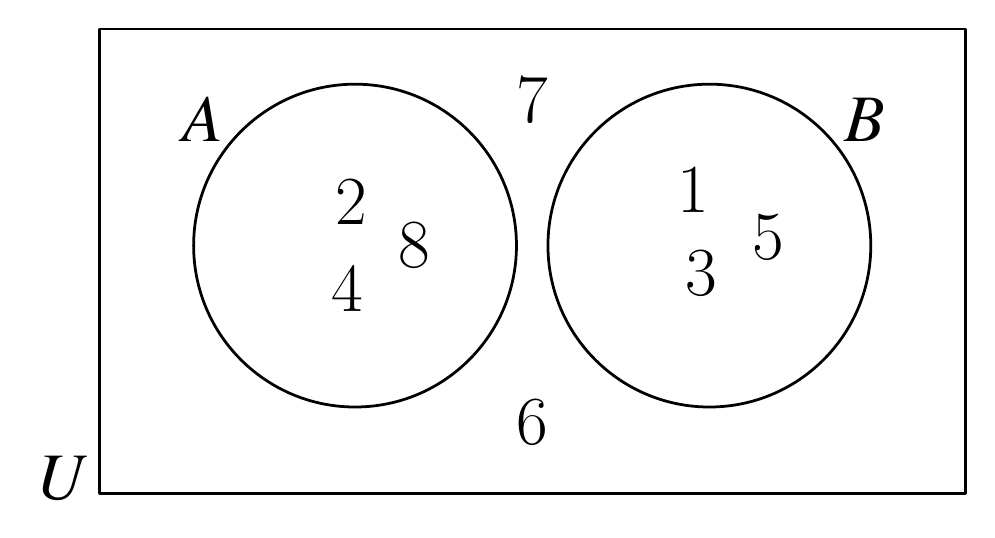
\begin{tikzpicture}[line cap=round,line join=round]

% --- geometry ---
    \def\R{2.05}                     % circle radius
    \coordinate (L)   at (-2.25,0.20); % left circle center (A)
    \coordinate (Rgt) at ( 2.25,0.20); % right circle center (B)

% universe rectangle
    \draw[line width=1.0pt] (-5.5,-2.95) rectangle (5.5,2.95);

% circles
    \draw[line width=1.0pt] (L) circle (\R);
    \draw[line width=1.0pt] (Rgt) circle (\R);

% labels
    \node[lab] at ($ (L) + (-1.95,1.60) $) {$A$};
    \node[lab] at ($ (Rgt) + ( 1.95,1.60) $) {$B$};

% numbers in A
    \node[lab] at ($ (L) + (-0.05,0.55) $) {2};
    \node[lab] at ($ (L) + (-0.10,-0.55) $) {4};
    \node[lab] at ($ (L) + ( 0.75,0.00) $) {8};

% numbers in B
    \node[lab] at ($ (Rgt) + (-0.20,0.70) $) {1};
    \node[lab] at ($ (Rgt) + (-0.10,-0.35) $) {3};
    \node[lab] at ($ (Rgt) + ( 0.75,0.10) $) {5};

% numbers outside circles (but inside U)
    \node[lab] at (0, 2.05) {7};
    \node[lab] at (0,-2.05) {6};

% universe label (outside bottom-left of the rectangle)
    \node[lab, anchor=north east] at (-5.5,-2.35) {$U$};

  \end{tikzpicture}
\end{document}